% Options for packages loaded elsewhere
\PassOptionsToPackage{unicode}{hyperref}
\PassOptionsToPackage{hyphens}{url}
\PassOptionsToPackage{dvipsnames,svgnames,x11names}{xcolor}
%
\documentclass[
  letterpaper,
  DIV=11,
  numbers=noendperiod]{scrartcl}

\usepackage{amsmath,amssymb}
\usepackage{lmodern}
\usepackage{iftex}
\ifPDFTeX
  \usepackage[T1]{fontenc}
  \usepackage[utf8]{inputenc}
  \usepackage{textcomp} % provide euro and other symbols
\else % if luatex or xetex
  \usepackage{unicode-math}
  \defaultfontfeatures{Scale=MatchLowercase}
  \defaultfontfeatures[\rmfamily]{Ligatures=TeX,Scale=1}
\fi
% Use upquote if available, for straight quotes in verbatim environments
\IfFileExists{upquote.sty}{\usepackage{upquote}}{}
\IfFileExists{microtype.sty}{% use microtype if available
  \usepackage[]{microtype}
  \UseMicrotypeSet[protrusion]{basicmath} % disable protrusion for tt fonts
}{}
\makeatletter
\@ifundefined{KOMAClassName}{% if non-KOMA class
  \IfFileExists{parskip.sty}{%
    \usepackage{parskip}
  }{% else
    \setlength{\parindent}{0pt}
    \setlength{\parskip}{6pt plus 2pt minus 1pt}}
}{% if KOMA class
  \KOMAoptions{parskip=half}}
\makeatother
\usepackage{xcolor}
\setlength{\emergencystretch}{3em} % prevent overfull lines
\setcounter{secnumdepth}{-\maxdimen} % remove section numbering
% Make \paragraph and \subparagraph free-standing
\ifx\paragraph\undefined\else
  \let\oldparagraph\paragraph
  \renewcommand{\paragraph}[1]{\oldparagraph{#1}\mbox{}}
\fi
\ifx\subparagraph\undefined\else
  \let\oldsubparagraph\subparagraph
  \renewcommand{\subparagraph}[1]{\oldsubparagraph{#1}\mbox{}}
\fi

\usepackage{color}
\usepackage{fancyvrb}
\newcommand{\VerbBar}{|}
\newcommand{\VERB}{\Verb[commandchars=\\\{\}]}
\DefineVerbatimEnvironment{Highlighting}{Verbatim}{commandchars=\\\{\}}
% Add ',fontsize=\small' for more characters per line
\usepackage{framed}
\definecolor{shadecolor}{RGB}{241,243,245}
\newenvironment{Shaded}{\begin{snugshade}}{\end{snugshade}}
\newcommand{\AlertTok}[1]{\textcolor[rgb]{0.68,0.00,0.00}{#1}}
\newcommand{\AnnotationTok}[1]{\textcolor[rgb]{0.37,0.37,0.37}{#1}}
\newcommand{\AttributeTok}[1]{\textcolor[rgb]{0.40,0.45,0.13}{#1}}
\newcommand{\BaseNTok}[1]{\textcolor[rgb]{0.68,0.00,0.00}{#1}}
\newcommand{\BuiltInTok}[1]{\textcolor[rgb]{0.00,0.23,0.31}{#1}}
\newcommand{\CharTok}[1]{\textcolor[rgb]{0.13,0.47,0.30}{#1}}
\newcommand{\CommentTok}[1]{\textcolor[rgb]{0.37,0.37,0.37}{#1}}
\newcommand{\CommentVarTok}[1]{\textcolor[rgb]{0.37,0.37,0.37}{\textit{#1}}}
\newcommand{\ConstantTok}[1]{\textcolor[rgb]{0.56,0.35,0.01}{#1}}
\newcommand{\ControlFlowTok}[1]{\textcolor[rgb]{0.00,0.23,0.31}{#1}}
\newcommand{\DataTypeTok}[1]{\textcolor[rgb]{0.68,0.00,0.00}{#1}}
\newcommand{\DecValTok}[1]{\textcolor[rgb]{0.68,0.00,0.00}{#1}}
\newcommand{\DocumentationTok}[1]{\textcolor[rgb]{0.37,0.37,0.37}{\textit{#1}}}
\newcommand{\ErrorTok}[1]{\textcolor[rgb]{0.68,0.00,0.00}{#1}}
\newcommand{\ExtensionTok}[1]{\textcolor[rgb]{0.00,0.23,0.31}{#1}}
\newcommand{\FloatTok}[1]{\textcolor[rgb]{0.68,0.00,0.00}{#1}}
\newcommand{\FunctionTok}[1]{\textcolor[rgb]{0.28,0.35,0.67}{#1}}
\newcommand{\ImportTok}[1]{\textcolor[rgb]{0.00,0.46,0.62}{#1}}
\newcommand{\InformationTok}[1]{\textcolor[rgb]{0.37,0.37,0.37}{#1}}
\newcommand{\KeywordTok}[1]{\textcolor[rgb]{0.00,0.23,0.31}{#1}}
\newcommand{\NormalTok}[1]{\textcolor[rgb]{0.00,0.23,0.31}{#1}}
\newcommand{\OperatorTok}[1]{\textcolor[rgb]{0.37,0.37,0.37}{#1}}
\newcommand{\OtherTok}[1]{\textcolor[rgb]{0.00,0.23,0.31}{#1}}
\newcommand{\PreprocessorTok}[1]{\textcolor[rgb]{0.68,0.00,0.00}{#1}}
\newcommand{\RegionMarkerTok}[1]{\textcolor[rgb]{0.00,0.23,0.31}{#1}}
\newcommand{\SpecialCharTok}[1]{\textcolor[rgb]{0.37,0.37,0.37}{#1}}
\newcommand{\SpecialStringTok}[1]{\textcolor[rgb]{0.13,0.47,0.30}{#1}}
\newcommand{\StringTok}[1]{\textcolor[rgb]{0.13,0.47,0.30}{#1}}
\newcommand{\VariableTok}[1]{\textcolor[rgb]{0.07,0.07,0.07}{#1}}
\newcommand{\VerbatimStringTok}[1]{\textcolor[rgb]{0.13,0.47,0.30}{#1}}
\newcommand{\WarningTok}[1]{\textcolor[rgb]{0.37,0.37,0.37}{\textit{#1}}}

\providecommand{\tightlist}{%
  \setlength{\itemsep}{0pt}\setlength{\parskip}{0pt}}\usepackage{longtable,booktabs,array}
\usepackage{calc} % for calculating minipage widths
% Correct order of tables after \paragraph or \subparagraph
\usepackage{etoolbox}
\makeatletter
\patchcmd\longtable{\par}{\if@noskipsec\mbox{}\fi\par}{}{}
\makeatother
% Allow footnotes in longtable head/foot
\IfFileExists{footnotehyper.sty}{\usepackage{footnotehyper}}{\usepackage{footnote}}
\makesavenoteenv{longtable}
\usepackage{graphicx}
\makeatletter
\def\maxwidth{\ifdim\Gin@nat@width>\linewidth\linewidth\else\Gin@nat@width\fi}
\def\maxheight{\ifdim\Gin@nat@height>\textheight\textheight\else\Gin@nat@height\fi}
\makeatother
% Scale images if necessary, so that they will not overflow the page
% margins by default, and it is still possible to overwrite the defaults
% using explicit options in \includegraphics[width, height, ...]{}
\setkeys{Gin}{width=\maxwidth,height=\maxheight,keepaspectratio}
% Set default figure placement to htbp
\makeatletter
\def\fps@figure{htbp}
\makeatother

\usepackage{fontspec}
\usepackage{multirow}
\usepackage{multicol}
\usepackage{colortbl}
\usepackage{hhline}
\newlength\Oldarrayrulewidth
\newlength\Oldtabcolsep
\usepackage{longtable}
\usepackage{array}
\usepackage{hyperref}
\usepackage{float}
\usepackage{wrapfig}
\KOMAoption{captions}{tableheading}
\makeatletter
\makeatother
\makeatletter
\makeatother
\makeatletter
\@ifpackageloaded{caption}{}{\usepackage{caption}}
\AtBeginDocument{%
\ifdefined\contentsname
  \renewcommand*\contentsname{Table of contents}
\else
  \newcommand\contentsname{Table of contents}
\fi
\ifdefined\listfigurename
  \renewcommand*\listfigurename{List of Figures}
\else
  \newcommand\listfigurename{List of Figures}
\fi
\ifdefined\listtablename
  \renewcommand*\listtablename{List of Tables}
\else
  \newcommand\listtablename{List of Tables}
\fi
\ifdefined\figurename
  \renewcommand*\figurename{Figure}
\else
  \newcommand\figurename{Figure}
\fi
\ifdefined\tablename
  \renewcommand*\tablename{Table}
\else
  \newcommand\tablename{Table}
\fi
}
\@ifpackageloaded{float}{}{\usepackage{float}}
\floatstyle{ruled}
\@ifundefined{c@chapter}{\newfloat{codelisting}{h}{lop}}{\newfloat{codelisting}{h}{lop}[chapter]}
\floatname{codelisting}{Listing}
\newcommand*\listoflistings{\listof{codelisting}{List of Listings}}
\makeatother
\makeatletter
\@ifpackageloaded{caption}{}{\usepackage{caption}}
\@ifpackageloaded{subcaption}{}{\usepackage{subcaption}}
\makeatother
\makeatletter
\@ifpackageloaded{tcolorbox}{}{\usepackage[many]{tcolorbox}}
\makeatother
\makeatletter
\@ifundefined{shadecolor}{\definecolor{shadecolor}{rgb}{.97, .97, .97}}
\makeatother
\makeatletter
\makeatother
\ifLuaTeX
  \usepackage{selnolig}  % disable illegal ligatures
\fi
\IfFileExists{bookmark.sty}{\usepackage{bookmark}}{\usepackage{hyperref}}
\IfFileExists{xurl.sty}{\usepackage{xurl}}{} % add URL line breaks if available
\urlstyle{same} % disable monospaced font for URLs
\hypersetup{
  pdftitle={Calibration Assignment},
  pdfauthor={Guillermo Romero \& Javier Patron},
  colorlinks=true,
  linkcolor={blue},
  filecolor={Maroon},
  citecolor={Blue},
  urlcolor={Blue},
  pdfcreator={LaTeX via pandoc}}

\title{Calibration Assignment}
\author{Guillermo Romero \& Javier Patron}
\date{}

\begin{document}
\maketitle
\ifdefined\Shaded\renewenvironment{Shaded}{\begin{tcolorbox}[frame hidden, borderline west={3pt}{0pt}{shadecolor}, interior hidden, breakable, enhanced, boxrule=0pt, sharp corners]}{\end{tcolorbox}}\fi

\begin{verbatim}
Warning: package 'ggplot2' was built under R version 4.2.3
\end{verbatim}

\begin{verbatim}
Warning: package 'tibble' was built under R version 4.2.3
\end{verbatim}

\begin{verbatim}
Warning: package 'dplyr' was built under R version 4.2.3
\end{verbatim}

\begin{verbatim}
-- Attaching core tidyverse packages ------------------------ tidyverse 2.0.0 --
v dplyr     1.1.2     v readr     2.1.4
v forcats   1.0.0     v stringr   1.5.0
v ggplot2   3.4.2     v tibble    3.2.1
v lubridate 1.9.2     v tidyr     1.3.0
v purrr     1.0.1     
-- Conflicts ------------------------------------------ tidyverse_conflicts() --
x dplyr::filter() masks stats::filter()
x dplyr::lag()    masks stats::lag()
i Use the conflicted package (<http://conflicted.r-lib.org/>) to force all conflicts to become errors
\end{verbatim}

\begin{verbatim}
Warning: package 'flextable' was built under R version 4.2.3
\end{verbatim}

\begin{verbatim}

Attaching package: 'flextable'

The following object is masked from 'package:purrr':

    compose

here() starts at C:/Users/bsf31/Documents/meds/ESM232_Examples
\end{verbatim}

\hypertarget{assignment}{%
\section{\texorpdfstring{\textbf{Assignment}}{Assignment}}\label{assignment}}

\begin{itemize}
\item
  \begin{quote}
  Part 1 from above: R function that codes a metric for performance
  evaluation

  \begin{itemize}
  \item
    must be a combination of at least two performance measures
  \item
    include some comments that explain `why' this metric
  \end{itemize}
  \end{quote}
\end{itemize}

This combined metric can be used to evaluate the model performance
considering both the discrepancy between the observed and modeled flow
values as well as the linear relationship between them.

Here's the reasoning behind this metric and an overview of the steps:

\textbf{Transformed Difference:} This measure captures the difference
between the observed and modeled flow values at the annual scale. By
calculating the difference between the sum of observed and modeled
values for each water year, we can assess how well the model is
reproducing the overall annual flow. The difference is then normalized
by the standard deviation of the differences to account for the
variations in the dataset and to have a comparable value across
different datasets.

\textbf{Correlation Coefficient:} This measure captures the linear
relationship between the observed and modeled flow values. A high
correlation coefficient indicates that the model is able to reproduce
the overall pattern of the flow values throughout the dataset.

\textbf{Combining the measures:} The transformed difference and
correlation coefficient are combined by calculating their arithmetic
mean. This provides a single value representing the model's performance,
considering both the discrepancy between observed and modeled flow
values and their linear relationship.

In summary, the combined\_metric function evaluates the performance of a
hydrologic model by considering both the difference between the observed
and modeled flow values at the annual scale and the linear relationship
between them. This combined metric can be used to compare the
performance of different models and assess how well they reproduce the
flow values in a given dataset.

\begin{Shaded}
\begin{Highlighting}[]
\NormalTok{combined\_metric }\OtherTok{\textless{}{-}} \ControlFlowTok{function}\NormalTok{(data) \{}
\NormalTok{  sager\_differences  }\OtherTok{\textless{}{-}}\NormalTok{ data }\SpecialCharTok{|\textgreater{}}
    \FunctionTok{group\_by}\NormalTok{(wy) }\SpecialCharTok{|\textgreater{}}
    \FunctionTok{summarize}\NormalTok{(}\AttributeTok{difference\_obs\_mod =} \FunctionTok{sum}\NormalTok{(model) }\SpecialCharTok{{-}} \FunctionTok{sum}\NormalTok{(obs))}
  
  \CommentTok{\# Calculate the mean difference}
\NormalTok{  mean\_difference }\OtherTok{\textless{}{-}} \FunctionTok{mean}\NormalTok{(sager\_differences}\SpecialCharTok{$}\NormalTok{difference\_obs\_mod)}
  
  \CommentTok{\# Calculate the standard deviation of the differences}
\NormalTok{  std\_dev\_difference }\OtherTok{\textless{}{-}} \FunctionTok{sd}\NormalTok{(sager\_differences}\SpecialCharTok{$}\NormalTok{difference\_obs\_mod)}
  
  \CommentTok{\# Compute the transformed difference (e.g., normalize by the standard deviation)}
\NormalTok{  sager\_differences }\OtherTok{\textless{}{-}}
\NormalTok{    sager\_differences }\SpecialCharTok{|\textgreater{}} \FunctionTok{mutate}\NormalTok{(}\AttributeTok{transformed\_diff =}\NormalTok{ difference\_obs\_mod }\SpecialCharTok{/}\NormalTok{ std\_dev\_difference)}
  
  \CommentTok{\# Compute the correlation coefficient between obs and model}
\NormalTok{  correlation\_coefficient }\OtherTok{\textless{}{-}} \FunctionTok{cor}\NormalTok{(data}\SpecialCharTok{$}\NormalTok{obs, data}\SpecialCharTok{$}\NormalTok{model)}
  
  \CommentTok{\# Combine the transformed difference and the correlation coefficient}
\NormalTok{  combined\_metric }\OtherTok{\textless{}{-}}
\NormalTok{    (}\FunctionTok{mean}\NormalTok{(sager\_differences}\SpecialCharTok{$}\NormalTok{transformed\_diff) }\SpecialCharTok{+}\NormalTok{ correlation\_coefficient) }\SpecialCharTok{/} \DecValTok{2}
  
\NormalTok{  combined\_metric}
\NormalTok{\}}
\end{Highlighting}
\end{Shaded}

\hypertarget{section}{%
\section{2}\label{section}}

\begin{itemize}
\item
  R markdown that does the following steps (with lots of documentation
  of the work flow):

  \begin{itemize}
  \item
    Part 2 from above:

    \begin{enumerate}
    \def\labelenumi{\arabic{enumi}.}
    \tightlist
    \item
      Apply your performance function to a subset of the Sagehen data
      set (with multiple simulations) that you want to use for
      calibration
    \end{enumerate}
  \end{itemize}
\end{itemize}

We perform a split-sample calibration using the year 1984 as the
calibration threshold. Then find the best parameter set and graph the
mean August streamflow for the best parameter set. Finally compute the
performance of the model using the best parameter set in pre and
post-calibration periods.

\begin{Shaded}
\begin{Highlighting}[]
\CommentTok{\# Read and organize the data}
\NormalTok{sager }\OtherTok{=} \FunctionTok{read.table}\NormalTok{(}\FunctionTok{here}\NormalTok{(}\StringTok{\textquotesingle{}data\textquotesingle{}}\NormalTok{,}\StringTok{"sager.txt"}\NormalTok{), }\AttributeTok{header=}\NormalTok{T)}

\CommentTok{\# add date}
\NormalTok{sager }\OtherTok{=}\NormalTok{ sager }\SpecialCharTok{\%\textgreater{}\%} \FunctionTok{mutate}\NormalTok{(}\AttributeTok{date =} \FunctionTok{paste}\NormalTok{(day,month,year, }\AttributeTok{sep=}\StringTok{"/"}\NormalTok{))}
\NormalTok{sager}\SpecialCharTok{$}\NormalTok{date }\OtherTok{=} \FunctionTok{as.Date}\NormalTok{(sager}\SpecialCharTok{$}\NormalTok{date,}\StringTok{"\%d/\%m/\%Y"}\NormalTok{)}

\CommentTok{\# Read and organize the data}
\NormalTok{sagerm }\OtherTok{\textless{}{-}} \FunctionTok{read.table}\NormalTok{(}\FunctionTok{here}\NormalTok{(}\StringTok{\textquotesingle{}data\textquotesingle{}}\NormalTok{,}\StringTok{"sagerm.txt"}\NormalTok{), }\AttributeTok{header =}\NormalTok{ T)}
\NormalTok{nsim }\OtherTok{\textless{}{-}} \FunctionTok{ncol}\NormalTok{(sagerm)}
\NormalTok{snames }\OtherTok{\textless{}{-}} \FunctionTok{sprintf}\NormalTok{(}\StringTok{"S\%d"}\NormalTok{, }\FunctionTok{seq}\NormalTok{(}\AttributeTok{from =} \DecValTok{1}\NormalTok{, }\AttributeTok{to =}\NormalTok{ nsim))}
\FunctionTok{colnames}\NormalTok{(sagerm) }\OtherTok{\textless{}{-}}\NormalTok{ snames}

\NormalTok{sagerm}\SpecialCharTok{$}\NormalTok{date }\OtherTok{\textless{}{-}}\NormalTok{ sager}\SpecialCharTok{$}\NormalTok{date}
\NormalTok{sagerm}\SpecialCharTok{$}\NormalTok{month }\OtherTok{\textless{}{-}}\NormalTok{ sager}\SpecialCharTok{$}\NormalTok{month}
\NormalTok{sagerm}\SpecialCharTok{$}\NormalTok{year }\OtherTok{\textless{}{-}}\NormalTok{ sager}\SpecialCharTok{$}\NormalTok{year}
\NormalTok{sagerm}\SpecialCharTok{$}\NormalTok{day }\OtherTok{\textless{}{-}}\NormalTok{ sager}\SpecialCharTok{$}\NormalTok{day}
\NormalTok{sagerm}\SpecialCharTok{$}\NormalTok{wy }\OtherTok{\textless{}{-}}\NormalTok{ sager}\SpecialCharTok{$}\NormalTok{wy}

\NormalTok{sagerm }\OtherTok{\textless{}{-}} \FunctionTok{left\_join}\NormalTok{(sagerm, sager[, }\FunctionTok{c}\NormalTok{(}\StringTok{"obs"}\NormalTok{, }\StringTok{"date"}\NormalTok{)], }\AttributeTok{by =} \FunctionTok{c}\NormalTok{(}\StringTok{"date"}\NormalTok{))}

\CommentTok{\# Split{-}sample calibration}
\NormalTok{calibration\_data }\OtherTok{\textless{}{-}} \FunctionTok{subset}\NormalTok{(sagerm, wy }\SpecialCharTok{\textless{}} \DecValTok{1984}\NormalTok{)}
\end{Highlighting}
\end{Shaded}

\begin{Shaded}
\begin{Highlighting}[]
\CommentTok{\# Define a function to compute the combined\_metric for each simulation}
\NormalTok{combined\_metric\_for\_simulation }\OtherTok{\textless{}{-}} \ControlFlowTok{function}\NormalTok{(sname, data, obs) \{}
\NormalTok{  model\_data }\OtherTok{\textless{}{-}}\NormalTok{ data[[sname]]}
\NormalTok{  wy\_data }\OtherTok{\textless{}{-}}\NormalTok{ data}\SpecialCharTok{$}\NormalTok{wy}
\NormalTok{  cm }\OtherTok{\textless{}{-}} \FunctionTok{combined\_metric}\NormalTok{(}\FunctionTok{data.frame}\NormalTok{(}\AttributeTok{obs =}\NormalTok{ obs, }\AttributeTok{model =}\NormalTok{ model\_data, }\AttributeTok{wy =}\NormalTok{ wy\_data))}
  \FunctionTok{return}\NormalTok{(}\FunctionTok{data.frame}\NormalTok{(}\AttributeTok{sim =}\NormalTok{ sname, }\AttributeTok{combined\_metric =}\NormalTok{ cm))}
\NormalTok{\}}


\CommentTok{\# Compute the combined\_metric for each simulation during the calibration period}
\NormalTok{res }\OtherTok{\textless{}{-}} \FunctionTok{map\_dfr}\NormalTok{(snames, combined\_metric\_for\_simulation, }\AttributeTok{data =}\NormalTok{ calibration\_data, }\AttributeTok{obs =}\NormalTok{ calibration\_data}\SpecialCharTok{$}\NormalTok{obs)}

\NormalTok{ft }\OtherTok{\textless{}{-}} \FunctionTok{flextable}\NormalTok{(}\FunctionTok{head}\NormalTok{(res))}

\FunctionTok{theme\_vader}\NormalTok{(ft)}
\end{Highlighting}
\end{Shaded}

\global\setlength{\Oldarrayrulewidth}{\arrayrulewidth}

\global\setlength{\Oldtabcolsep}{\tabcolsep}

\setlength{\tabcolsep}{0pt}

\renewcommand*{\arraystretch}{1.5}



\providecommand{\ascline}[3]{\noalign{\global\arrayrulewidth #1}\arrayrulecolor[HTML]{#2}\cline{#3}}

\begin{longtable}[c]{|p{0.75in}|p{0.75in}}



\hhline{>{\arrayrulecolor[HTML]{000000}\global\arrayrulewidth=0pt}->{\arrayrulecolor[HTML]{000000}\global\arrayrulewidth=0pt}-}

\multicolumn{1}{>{\cellcolor[HTML]{242424}\raggedright}m{\dimexpr 0.75in+0\tabcolsep}}{\textcolor[HTML]{DFDFDF}{\fontsize{11}{11}\selectfont{\textbf{sim}}}} & \multicolumn{1}{>{\cellcolor[HTML]{242424}\raggedleft}m{\dimexpr 0.75in+0\tabcolsep}}{\textcolor[HTML]{DFDFDF}{\fontsize{11}{11}\selectfont{\textbf{combined\_metric}}}} \\

\noalign{\global\arrayrulewidth 0pt}\arrayrulecolor[HTML]{000000}

\hhline{>{\arrayrulecolor[HTML]{FF0000}\global\arrayrulewidth=1.5pt}->{\arrayrulecolor[HTML]{FF0000}\global\arrayrulewidth=1.5pt}-}\endhead



\multicolumn{1}{>{\cellcolor[HTML]{242424}\raggedright}m{\dimexpr 0.75in+0\tabcolsep}}{\textcolor[HTML]{DFDFDF}{\fontsize{11}{11}\selectfont{S1}}} & \multicolumn{1}{>{\cellcolor[HTML]{242424}\raggedleft}m{\dimexpr 0.75in+0\tabcolsep}}{\textcolor[HTML]{DFDFDF}{\fontsize{11}{11}\selectfont{0.49701896}}} \\

\noalign{\global\arrayrulewidth 0pt}\arrayrulecolor[HTML]{000000}





\multicolumn{1}{>{\cellcolor[HTML]{242424}\raggedright}m{\dimexpr 0.75in+0\tabcolsep}}{\textcolor[HTML]{DFDFDF}{\fontsize{11}{11}\selectfont{S2}}} & \multicolumn{1}{>{\cellcolor[HTML]{242424}\raggedleft}m{\dimexpr 0.75in+0\tabcolsep}}{\textcolor[HTML]{DFDFDF}{\fontsize{11}{11}\selectfont{0.52936977}}} \\

\noalign{\global\arrayrulewidth 0pt}\arrayrulecolor[HTML]{000000}





\multicolumn{1}{>{\cellcolor[HTML]{242424}\raggedright}m{\dimexpr 0.75in+0\tabcolsep}}{\textcolor[HTML]{DFDFDF}{\fontsize{11}{11}\selectfont{S3}}} & \multicolumn{1}{>{\cellcolor[HTML]{242424}\raggedleft}m{\dimexpr 0.75in+0\tabcolsep}}{\textcolor[HTML]{DFDFDF}{\fontsize{11}{11}\selectfont{-0.50282226}}} \\

\noalign{\global\arrayrulewidth 0pt}\arrayrulecolor[HTML]{000000}





\multicolumn{1}{>{\cellcolor[HTML]{242424}\raggedright}m{\dimexpr 0.75in+0\tabcolsep}}{\textcolor[HTML]{DFDFDF}{\fontsize{11}{11}\selectfont{S4}}} & \multicolumn{1}{>{\cellcolor[HTML]{242424}\raggedleft}m{\dimexpr 0.75in+0\tabcolsep}}{\textcolor[HTML]{DFDFDF}{\fontsize{11}{11}\selectfont{-0.14164949}}} \\

\noalign{\global\arrayrulewidth 0pt}\arrayrulecolor[HTML]{000000}





\multicolumn{1}{>{\cellcolor[HTML]{242424}\raggedright}m{\dimexpr 0.75in+0\tabcolsep}}{\textcolor[HTML]{DFDFDF}{\fontsize{11}{11}\selectfont{S5}}} & \multicolumn{1}{>{\cellcolor[HTML]{242424}\raggedleft}m{\dimexpr 0.75in+0\tabcolsep}}{\textcolor[HTML]{DFDFDF}{\fontsize{11}{11}\selectfont{-0.04141438}}} \\

\noalign{\global\arrayrulewidth 0pt}\arrayrulecolor[HTML]{000000}





\multicolumn{1}{>{\cellcolor[HTML]{242424}\raggedright}m{\dimexpr 0.75in+0\tabcolsep}}{\textcolor[HTML]{DFDFDF}{\fontsize{11}{11}\selectfont{S6}}} & \multicolumn{1}{>{\cellcolor[HTML]{242424}\raggedleft}m{\dimexpr 0.75in+0\tabcolsep}}{\textcolor[HTML]{DFDFDF}{\fontsize{11}{11}\selectfont{-0.45896335}}} \\

\noalign{\global\arrayrulewidth 0pt}\arrayrulecolor[HTML]{000000}





\end{longtable}



\arrayrulecolor[HTML]{000000}

\global\setlength{\arrayrulewidth}{\Oldarrayrulewidth}

\global\setlength{\tabcolsep}{\Oldtabcolsep}

\renewcommand*{\arraystretch}{1}

\begin{Shaded}
\begin{Highlighting}[]
\CommentTok{\# Find the best and worst parameter sets}
\NormalTok{best\_parameter }\OtherTok{\textless{}{-}}\NormalTok{ res }\SpecialCharTok{\%\textgreater{}\%} \FunctionTok{slice\_max}\NormalTok{(combined\_metric) }\SpecialCharTok{|\textgreater{}} \FunctionTok{mutate}\NormalTok{(}\AttributeTok{parameter\_type =} \StringTok{\textquotesingle{}best\textquotesingle{}}\NormalTok{, }\AttributeTok{.before =}\NormalTok{ sim)}
\NormalTok{worst\_parameter }\OtherTok{\textless{}{-}}\NormalTok{ res }\SpecialCharTok{\%\textgreater{}\%} \FunctionTok{slice\_min}\NormalTok{(combined\_metric) }\SpecialCharTok{|\textgreater{}} \FunctionTok{mutate}\NormalTok{(}\AttributeTok{parameter\_type =} \StringTok{\textquotesingle{}worst\textquotesingle{}}\NormalTok{, }\AttributeTok{.before =}\NormalTok{ sim)}

\NormalTok{params }\OtherTok{\textless{}{-}} \FunctionTok{bind\_rows}\NormalTok{(best\_parameter,worst\_parameter) }\SpecialCharTok{|\textgreater{}} 
  \FunctionTok{flextable}\NormalTok{()}

\FunctionTok{theme\_vader}\NormalTok{(params)}
\end{Highlighting}
\end{Shaded}

\global\setlength{\Oldarrayrulewidth}{\arrayrulewidth}

\global\setlength{\Oldtabcolsep}{\tabcolsep}

\setlength{\tabcolsep}{0pt}

\renewcommand*{\arraystretch}{1.5}



\providecommand{\ascline}[3]{\noalign{\global\arrayrulewidth #1}\arrayrulecolor[HTML]{#2}\cline{#3}}

\begin{longtable}[c]{|p{0.75in}|p{0.75in}|p{0.75in}}



\hhline{>{\arrayrulecolor[HTML]{000000}\global\arrayrulewidth=0pt}->{\arrayrulecolor[HTML]{000000}\global\arrayrulewidth=0pt}->{\arrayrulecolor[HTML]{000000}\global\arrayrulewidth=0pt}-}

\multicolumn{1}{>{\cellcolor[HTML]{242424}\raggedright}m{\dimexpr 0.75in+0\tabcolsep}}{\textcolor[HTML]{DFDFDF}{\fontsize{11}{11}\selectfont{\textbf{parameter\_type}}}} & \multicolumn{1}{>{\cellcolor[HTML]{242424}\raggedright}m{\dimexpr 0.75in+0\tabcolsep}}{\textcolor[HTML]{DFDFDF}{\fontsize{11}{11}\selectfont{\textbf{sim}}}} & \multicolumn{1}{>{\cellcolor[HTML]{242424}\raggedleft}m{\dimexpr 0.75in+0\tabcolsep}}{\textcolor[HTML]{DFDFDF}{\fontsize{11}{11}\selectfont{\textbf{combined\_metric}}}} \\

\noalign{\global\arrayrulewidth 0pt}\arrayrulecolor[HTML]{000000}

\hhline{>{\arrayrulecolor[HTML]{FF0000}\global\arrayrulewidth=1.5pt}->{\arrayrulecolor[HTML]{FF0000}\global\arrayrulewidth=1.5pt}->{\arrayrulecolor[HTML]{FF0000}\global\arrayrulewidth=1.5pt}-}\endhead



\multicolumn{1}{>{\cellcolor[HTML]{242424}\raggedright}m{\dimexpr 0.75in+0\tabcolsep}}{\textcolor[HTML]{DFDFDF}{\fontsize{11}{11}\selectfont{best}}} & \multicolumn{1}{>{\cellcolor[HTML]{242424}\raggedright}m{\dimexpr 0.75in+0\tabcolsep}}{\textcolor[HTML]{DFDFDF}{\fontsize{11}{11}\selectfont{S49}}} & \multicolumn{1}{>{\cellcolor[HTML]{242424}\raggedleft}m{\dimexpr 0.75in+0\tabcolsep}}{\textcolor[HTML]{DFDFDF}{\fontsize{11}{11}\selectfont{1.0406890}}} \\

\noalign{\global\arrayrulewidth 0pt}\arrayrulecolor[HTML]{000000}





\multicolumn{1}{>{\cellcolor[HTML]{242424}\raggedright}m{\dimexpr 0.75in+0\tabcolsep}}{\textcolor[HTML]{DFDFDF}{\fontsize{11}{11}\selectfont{worst}}} & \multicolumn{1}{>{\cellcolor[HTML]{242424}\raggedright}m{\dimexpr 0.75in+0\tabcolsep}}{\textcolor[HTML]{DFDFDF}{\fontsize{11}{11}\selectfont{S43}}} & \multicolumn{1}{>{\cellcolor[HTML]{242424}\raggedleft}m{\dimexpr 0.75in+0\tabcolsep}}{\textcolor[HTML]{DFDFDF}{\fontsize{11}{11}\selectfont{-0.5680795}}} \\

\noalign{\global\arrayrulewidth 0pt}\arrayrulecolor[HTML]{000000}





\end{longtable}



\arrayrulecolor[HTML]{000000}

\global\setlength{\arrayrulewidth}{\Oldarrayrulewidth}

\global\setlength{\tabcolsep}{\Oldtabcolsep}

\renewcommand*{\arraystretch}{1}

\begin{Shaded}
\begin{Highlighting}[]
\FunctionTok{ggthemr}\NormalTok{(}\StringTok{\textquotesingle{}flat dark\textquotesingle{}}\NormalTok{, }\AttributeTok{type =} \StringTok{\textquotesingle{}outer\textquotesingle{}}\NormalTok{, }\AttributeTok{layout =} \StringTok{"scientific"}\NormalTok{)}
\end{Highlighting}
\end{Shaded}

\begin{Shaded}
\begin{Highlighting}[]
\CommentTok{\# Compare the performance of the best and worst parameter sets}
\NormalTok{comparison\_data }\OtherTok{\textless{}{-}}\NormalTok{ sagerm }\SpecialCharTok{\%\textgreater{}\%}
  \FunctionTok{select}\NormalTok{(}\FunctionTok{c}\NormalTok{(best\_parameter}\SpecialCharTok{$}\NormalTok{sim, worst\_parameter}\SpecialCharTok{$}\NormalTok{sim), date, obs, month, day, year, wy)}

\NormalTok{comparison\_data\_mwy }\OtherTok{\textless{}{-}}\NormalTok{ comparison\_data }\SpecialCharTok{\%\textgreater{}\%}
  \FunctionTok{select}\NormalTok{(}\SpecialCharTok{{-}}\FunctionTok{c}\NormalTok{(day, date, year)) }\SpecialCharTok{\%\textgreater{}\%}
  \FunctionTok{group\_by}\NormalTok{(month, wy) }\SpecialCharTok{\%\textgreater{}\%}
  \FunctionTok{summarize}\NormalTok{(}\FunctionTok{across}\NormalTok{(}\FunctionTok{everything}\NormalTok{(), mean))}
\end{Highlighting}
\end{Shaded}

\begin{verbatim}
`summarise()` has grouped output by 'month'. You can override using the
`.groups` argument.
\end{verbatim}

\begin{Shaded}
\begin{Highlighting}[]
\NormalTok{comparison\_data\_mwyl }\OtherTok{\textless{}{-}}\NormalTok{ comparison\_data\_mwy }\SpecialCharTok{\%\textgreater{}\%}
  \FunctionTok{pivot\_longer}\NormalTok{(}\AttributeTok{cols =} \SpecialCharTok{!}\FunctionTok{c}\NormalTok{(month, wy), }\AttributeTok{names\_to =} \StringTok{"sim"}\NormalTok{, }\AttributeTok{values\_to =} \StringTok{"flow"}\NormalTok{)}
\end{Highlighting}
\end{Shaded}

\begin{Shaded}
\begin{Highlighting}[]
\FunctionTok{ggplot}\NormalTok{(}\FunctionTok{subset}\NormalTok{(comparison\_data\_mwyl, month }\SpecialCharTok{==} \DecValTok{8}\NormalTok{), }\FunctionTok{aes}\NormalTok{(sim, flow)) }\SpecialCharTok{+} \FunctionTok{geom\_boxplot}\NormalTok{()}
\end{Highlighting}
\end{Shaded}

\begin{figure}[H]

{\centering 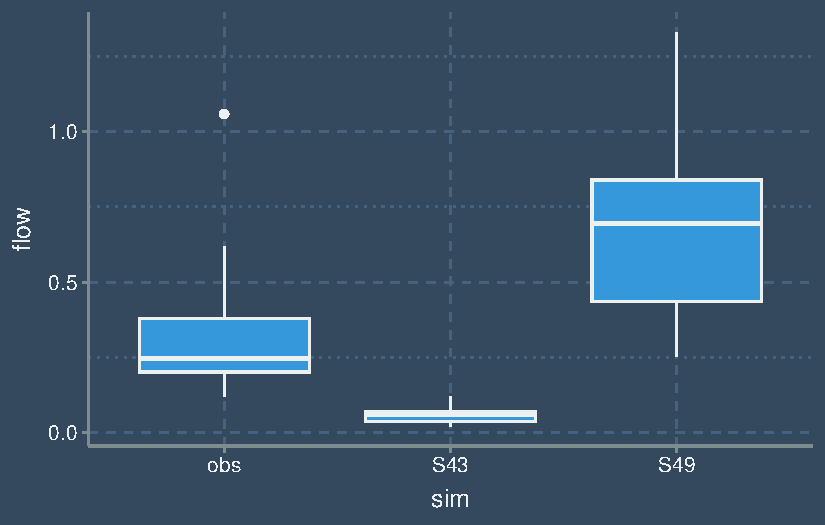
\includegraphics{calibration-assignment_files/figure-pdf/unnamed-chunk-8-1.pdf}

}

\end{figure}

\begin{verbatim}
2.  Summarize the performance over the calibration period in 1-2 graphs; you can decide what is useful
\end{verbatim}

\begin{Shaded}
\begin{Highlighting}[]
\CommentTok{\# Apply the best parameter set to the validation data}
\NormalTok{best\_sim }\OtherTok{\textless{}{-}}\NormalTok{ best\_parameter}\SpecialCharTok{$}\NormalTok{sim}
\NormalTok{validation\_data }\OtherTok{\textless{}{-}} \FunctionTok{subset}\NormalTok{(sagerm, wy }\SpecialCharTok{\textgreater{}=} \DecValTok{1984}\NormalTok{)}

\NormalTok{validation\_data\_adjusted }\OtherTok{\textless{}{-}}\NormalTok{ validation\_data }\SpecialCharTok{\%\textgreater{}\%}
  \FunctionTok{mutate}\NormalTok{(}\AttributeTok{model =} \SpecialCharTok{!!}\FunctionTok{sym}\NormalTok{(best\_sim))}

\CommentTok{\# Plot the mean August streamflow for the best parameter set}
\NormalTok{mean\_august\_streamflow }\OtherTok{\textless{}{-}}\NormalTok{ validation\_data\_adjusted }\SpecialCharTok{\%\textgreater{}\%}
  \FunctionTok{filter}\NormalTok{(month }\SpecialCharTok{==} \DecValTok{8}\NormalTok{) }\SpecialCharTok{\%\textgreater{}\%}
  \FunctionTok{group\_by}\NormalTok{(year) }\SpecialCharTok{\%\textgreater{}\%}
  \FunctionTok{summarize}\NormalTok{(}\AttributeTok{mean\_obs =} \FunctionTok{mean}\NormalTok{(obs),}
            \AttributeTok{mean\_model =} \FunctionTok{mean}\NormalTok{(model))}
\end{Highlighting}
\end{Shaded}

\begin{Shaded}
\begin{Highlighting}[]
\FunctionTok{ggplot}\NormalTok{(mean\_august\_streamflow, }\FunctionTok{aes}\NormalTok{(}\AttributeTok{x =}\NormalTok{ year)) }\SpecialCharTok{+}
  \FunctionTok{geom\_line}\NormalTok{(}\FunctionTok{aes}\NormalTok{(}\AttributeTok{y =}\NormalTok{ mean\_obs, }\AttributeTok{color =} \StringTok{"Observed"}\NormalTok{)) }\SpecialCharTok{+}
  \FunctionTok{geom\_line}\NormalTok{(}\FunctionTok{aes}\NormalTok{(}\AttributeTok{y =}\NormalTok{ mean\_model, }\AttributeTok{color =} \StringTok{"Adjusted Model"}\NormalTok{))}\SpecialCharTok{+}
  \FunctionTok{labs}\NormalTok{(}\AttributeTok{title =} \StringTok{"Mean August Streamflow"}\NormalTok{,}
       \AttributeTok{x =} \StringTok{"Year"}\NormalTok{,}
       \AttributeTok{y =} \StringTok{"Streamflow"}\NormalTok{,}
       \AttributeTok{color =} \StringTok{"Data"}\NormalTok{)}
\end{Highlighting}
\end{Shaded}

\begin{figure}[H]

{\centering 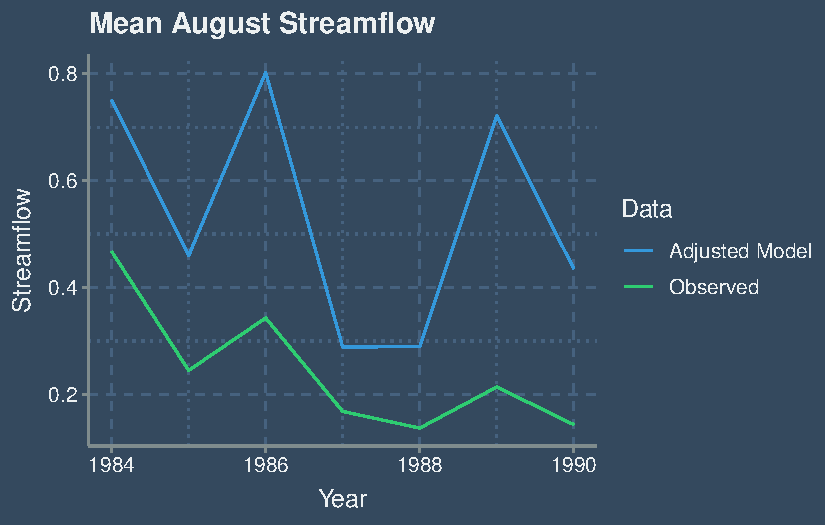
\includegraphics{calibration-assignment_files/figure-pdf/unnamed-chunk-10-1.pdf}

}

\end{figure}

\begin{Shaded}
\begin{Highlighting}[]
\CommentTok{\# Plot the performance over the calibration period}
\FunctionTok{ggplot}\NormalTok{(res, }\FunctionTok{aes}\NormalTok{(}\AttributeTok{x =}\NormalTok{ sim, }\AttributeTok{y =}\NormalTok{ combined\_metric, }\AttributeTok{color =}\NormalTok{ combined\_metric)) }\SpecialCharTok{+}
  \FunctionTok{geom\_point}\NormalTok{() }\SpecialCharTok{+}
  \FunctionTok{scale\_color\_gradient2}\NormalTok{(}\AttributeTok{low =} \StringTok{"blue"}\NormalTok{, }\AttributeTok{mid =} \StringTok{"white"}\NormalTok{, }\AttributeTok{high =} \StringTok{"red"}\NormalTok{, }\AttributeTok{midpoint =} \FunctionTok{median}\NormalTok{(res}\SpecialCharTok{$}\NormalTok{combined\_metric)) }\SpecialCharTok{+}
  \FunctionTok{scale\_x\_discrete}\NormalTok{(}\AttributeTok{breaks =} \FunctionTok{seq}\NormalTok{(}\AttributeTok{from =} \DecValTok{1}\NormalTok{, }\AttributeTok{to =} \FunctionTok{length}\NormalTok{(snames), }\AttributeTok{by =} \DecValTok{10}\NormalTok{), }\AttributeTok{labels =}\NormalTok{ snames[}\FunctionTok{seq}\NormalTok{(}\AttributeTok{from =} \DecValTok{1}\NormalTok{, }\AttributeTok{to =} \FunctionTok{length}\NormalTok{(snames), }\AttributeTok{by =} \DecValTok{10}\NormalTok{)]) }\SpecialCharTok{+}
  \FunctionTok{labs}\NormalTok{(}\AttributeTok{title =} \StringTok{"Model Performance Over Calibration Period"}\NormalTok{,}
       \AttributeTok{x =} \StringTok{"Simulation"}\NormalTok{,}
       \AttributeTok{y =} \StringTok{"Combined Metric"}\NormalTok{,}
       \AttributeTok{color =} \StringTok{"Combined Metric"}\NormalTok{)}
\end{Highlighting}
\end{Shaded}

\begin{figure}[H]

{\centering 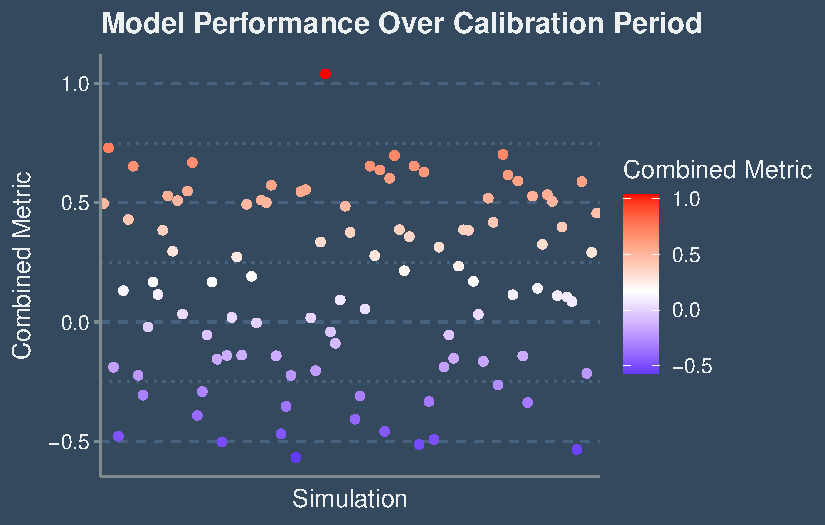
\includegraphics{calibration-assignment_files/figure-pdf/unnamed-chunk-11-1.pdf}

}

\end{figure}

\begin{Shaded}
\begin{Highlighting}[]
\CommentTok{\# Compute the performance of the model using the best parameter set in pre and post{-}calibration periods}
\NormalTok{pre\_calibration\_performance }\OtherTok{\textless{}{-}} \FunctionTok{combined\_metric}\NormalTok{(calibration\_data }\SpecialCharTok{\%\textgreater{}\%} \FunctionTok{mutate}\NormalTok{(}\AttributeTok{model =} \SpecialCharTok{!!}\FunctionTok{sym}\NormalTok{(best\_sim)))}
\NormalTok{post\_calibration\_performance }\OtherTok{\textless{}{-}} \FunctionTok{combined\_metric}\NormalTok{(validation\_data\_adjusted)}

\NormalTok{performance\_change }\OtherTok{\textless{}{-}}\NormalTok{ post\_calibration\_performance }\SpecialCharTok{{-}}\NormalTok{ pre\_calibration\_performance}
\NormalTok{performance\_change}
\end{Highlighting}
\end{Shaded}

\begin{verbatim}
[1] -0.09090848
\end{verbatim}

\begin{verbatim}
    3.  Record your 'best' and 'worst' parameter set in this [spreadsheet](https://docs.google.com/spreadsheets/d/1444ILTaP6pcqvudQopZZVP2WDDJ1NNgXX6sdPdwdbXE/edit#gid=0) and in your Rmd
\end{verbatim}



\end{document}
